% answers.tex —— 2006 年·四川卷·理科 · 参考答案与详细解析片段
% 由 tools/generate_projects.py 依来源总账自 2006/2006_数学真题_四川理_试题.md + 2006/2006_数学真题_四川理_解析正文.md + 2006/2006_数学真题_四川理_答案要点.md 生成，勿手改（改源 MD 后重跑）


\begin{gktip}
以下解答依据固定 PDF 可见题面推导，不是卷内答案或官方解析。固定副本的发布者、版次、来源链及官方身份未核。
\end{gktip}

\begin{answer}
\gksolhead{1}{}

\textbf{题目}：

已知集合 $A=\{x\mid x^2-5x+6\leqslant0\}$，集合 $B=\{x\mid |2x-1|>3\}$，则集合 $A\cap B=$\mbox{（　　）}。

（A）$\{x\mid 2\leqslant x\leqslant3\}$　　（B）$\{x\mid 2\leqslant x<3\}$

（C）$\{x\mid 2<x\leqslant3\}$　　（D）$\{x\mid -1<x<3\}$

\Needspace{4\baselineskip}
\textbf{解析}

$(x-2)(x-3)\leqslant0$，故 $A=[2,3]$；$|2x-1|>3$ 等价于 $x<-1$ 或 $x>2$。因此 $A\cap B=(2,3]$。

\gkanswer{答案：C}

\end{answer}
\begin{answer}
\gksolhead{2}{}

\textbf{题目}：

复数 $(1-i)^3$ 的虚部为\mbox{（　　）}。

（A）$3$　　（B）$-3$　　（C）$2$　　（D）$-2$

\Needspace{4\baselineskip}
\textbf{解析}

$(1-i)^2=-2i$，所以 $(1-i)^3=-2-2i$，虚部为 $-2$。

\gkanswer{答案：D}

\end{answer}
\begin{answer}
\gksolhead{3}{}

\textbf{题目}：

\Needspace{5\baselineskip}
已知
\nopagebreak[4]
\[
f(x)=
\begin{cases}
2x+3,&x\ne1,\\
2,&x=1,
\end{cases}
\]
下面结论正确的是\mbox{（　　）}。

（A）$f(x)$ 在 $x=1$ 处连续　　（B）$f(1)=5$

（C）$\displaystyle\lim_{x\to1^-}f(x)=2$　　（D）$\displaystyle\lim_{x\to1^+}f(x)=5$

\Needspace{4\baselineskip}
\textbf{解析}

当 $x\ne1$ 时 $f(x)=2x+3$，故 $\lim_{x\to1^-}f(x)=\lim_{x\to1^+}f(x)=5$，但 $f(1)=2$。只有 D 正确。

\gkanswer{答案：D}

\end{answer}
\begin{answer}
\gksolhead{4}{}

\textbf{题目}：

已知二面角 $\alpha-l-\beta$ 的大小为 $60^\circ$，$m,n$ 为异面直线，且 $m\perp\alpha$，$n\perp\beta$，则 $m,n$ 所成的角为\mbox{（　　）}。

（A）$30^\circ$　　（B）$60^\circ$　　（C）$90^\circ$　　（D）$120^\circ$

\Needspace{4\baselineskip}
\textbf{解析}

两条直线的方向分别垂直于 $\alpha\text{、}\beta$，夹角的锐角或直角值与两平面法线夹角相同。由二面角为 $60^\circ$，两直线所成的角为 $60^\circ$。

\gkanswer{答案：B}

\end{answer}
\begin{answer}
\gksolhead{5}{}

\textbf{题目}：

下列函数中，图象的一部分如图所示的是\mbox{（　　）}。
\nopagebreak[4]
\begin{center}% 2006 四川理科 Q5：按印刷页332题图重用同源三角函数曲线。
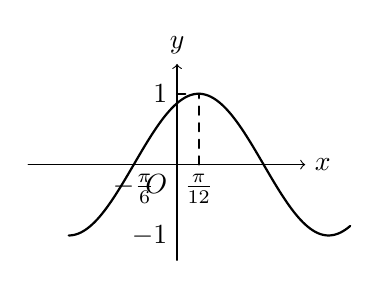
\begin{tikzpicture}[line cap=round,line join=round,x=1.05cm,y=0.9cm]
  \draw[->] (-1.8,0)--(1.55,0) node[right] {$x$};
  \draw[->] (0,-1.35)--(0,1.42) node[above] {$y$};
  \draw[thick,dashed] ({pi/12},0)--({pi/12},1);
  \draw[thick,dashed] (0,1)--({pi/12},1);
  \draw[thick,domain=-75:120,samples=120,variable=\t]
    plot ({\t*pi/180},{cos(2*\t-30)});
  \node[below left] at (0,0) {$O$};
  \node[left] at (0,1) {$1$};
  \node[left] at (0,-1) {$-1$};
  \node[below] at ({-pi/6},0) {$-\frac{\pi}{6}$};
  \node[below] at ({pi/12},0) {$\frac{\pi}{12}$};
\end{tikzpicture}
\end{center}
\nopagebreak[4]
（A）$y=\sin\left(x+\dfrac\pi6\right)$　　（B）$y=\sin\left(2x-\dfrac\pi6\right)$

（C）$y=\cos\left(4x-\dfrac\pi3\right)$　　（D）$y=\cos\left(2x-\dfrac\pi6\right)$

\Needspace{4\baselineskip}
\textbf{解析}

图象在 $x=\dfrac\pi{12}$ 处取最大值 $1$，且 $x=-\dfrac\pi6$ 为零点，符合 $y=\cos\left(2x-\dfrac\pi6\right)$。

\gkanswer{答案：D}

\end{answer}
\begin{answer}
\gksolhead{6}{}

\textbf{题目}：

已知两定点 $A(-2,0)$、$B(1,0)$，如果动点 $P$ 满足 $|PA|=2|PB|$，则点 $P$ 的轨迹所包围的图形的面积等于\mbox{（　　）}。

（A）$\pi$　　（B）$4\pi$　　（C）$8\pi$　　（D）$9\pi$

\Needspace{4\baselineskip}
\textbf{解析}

由 $|PA|=2|PB|$，平方得 $(x+2)^2+y^2=4((x-1)^2+y^2)$，化为 $(x-2)^2+y^2=4$。轨迹围成半径为 $2$ 的圆，面积为 $4\pi$。

\gkanswer{答案：B}

\end{answer}
\begin{answer}
\gksolhead{7}{}

\textbf{题目}：

如图，已知正六边形 $P_1P_2P_3P_4P_5P_6$，下列向量的数量积中最大的是\mbox{（　　）}。
\nopagebreak[4]
\begin{center}% 2006 四川理科 Q7：正六边形顶点顺序与印刷页332一致。
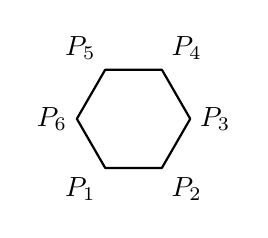
\begin{tikzpicture}[line cap=round,line join=round,x=0.72cm,y=0.72cm]
  \coordinate (P1) at (0,0);
  \coordinate (P2) at (1,0);
  \coordinate (P3) at (1.5,0.866);
  \coordinate (P4) at (1,1.732);
  \coordinate (P5) at (0,1.732);
  \coordinate (P6) at (-0.5,0.866);
  \draw[thick] (P1)--(P2)--(P3)--(P4)--(P5)--(P6)--cycle;
  \node[below left] at (P1) {$P_1$};
  \node[below right] at (P2) {$P_2$};
  \node[right] at (P3) {$P_3$};
  \node[above right] at (P4) {$P_4$};
  \node[above left] at (P5) {$P_5$};
  \node[left] at (P6) {$P_6$};
\end{tikzpicture}
\end{center}
\nopagebreak[4]
（A）$\overrightarrow{P_1P_2}\cdot\overrightarrow{P_1P_3}$　　（B）$\overrightarrow{P_1P_2}\cdot\overrightarrow{P_1P_4}$

（C）$\overrightarrow{P_1P_2}\cdot\overrightarrow{P_1P_5}$　　（D）$\overrightarrow{P_1P_2}\cdot\overrightarrow{P_1P_6}$

\Needspace{4\baselineskip}
\textbf{解析}

设正六边形边长为 $s$，按原图令 $\overrightarrow{P_1P_2}=(s,0)$。则四个选项中的点积依次为 $\frac32s^2\text{、}s^2\text{、}0\text{、}-\frac12s^2$，最大值对应 A。

\gkanswer{答案：A}

\end{answer}
\begin{answer}
\gksolhead{8}{}

\textbf{题目}：

某厂生产甲产品每千克需用原料 $A$ 和原料 $B$ 分别为 $a_1\text{、}b_1$ 千克，生产乙产品每千克需用原料 $A$ 和原料 $B$ 分别为 $a_2\text{、}b_2$ 千克。甲、乙产品每千克可获利润分别为 $d_1\text{、}d_2$ 元。月初一次性购进本月用原料 $A\text{、}B$ 各 $c_1\text{、}c_2$ 千克。要计划本月生产甲产品和乙产品各多少千克才能使月利润总额达到最大。在这个问题中，设全月生产甲、乙两种产品分别为 $x$ 千克、$y$ 千克，月利润总额为 $z$ 元，那么，用于求使总利润 $z=d_1x+d_2y$ 最大的数学模型中，约束条件为\mbox{（　　）}。

（A）$\begin{cases}a_1x+a_2y\geqslant c_1,\\b_1x+b_2y\geqslant c_2,\\x\geqslant0,\\y\geqslant0\end{cases}$　　（B）$\begin{cases}a_1x+b_1y\leqslant c_1,\\a_2x+b_2y\leqslant c_2,\\x\geqslant0,\\y\geqslant0\end{cases}$

（C）$\begin{cases}a_1x+a_2y\leqslant c_1,\\b_1x+b_2y\leqslant c_2,\\x\geqslant0,\\y\geqslant0\end{cases}$　　（D）$\begin{cases}a_1x+a_2y=c_1,\\b_1x+b_2y=c_2,\\x\geqslant0,\\y\geqslant0\end{cases}$

\Needspace{4\baselineskip}
\textbf{解析}

令甲、乙产品产量分别为 $x,y$。原料 $A$、$B$ 的总用量分别是 $a_1x+a_2y$ 与 $b_1x+b_2y$，均不能超过库存 $c_1,c_2$；同时 $x,y\geqslant0$。因此约束组为 C。

\gkanswer{答案：C}

\end{answer}
\begin{answer}
\gksolhead{9}{}

\textbf{题目}：

直线 $y=x-3$ 与抛物线 $y^2=4x$ 交于 $A\text{、}B$ 两点，过 $A\text{、}B$ 两点向抛物线的准线作垂线，垂足分别为 $P\text{、}Q$，则梯形 $APQB$ 的面积为\mbox{（　　）}。

（A）$48$　　（B）$56$　　（C）$64$　　（D）$72$

\Needspace{4\baselineskip}
\textbf{解析}

联立 $y=x-3$ 与 $y^2=4x$，得交点 $(1,-2)\text{、}(9,6)$。抛物线准线为 $x=-1$，故 $AP=2\text{、}BQ=10$；两平行边间距为 $6-(-2)=8$。梯形面积为 $\frac{2+10}{2}\cdot8=48$。

\gkanswer{答案：A}

\end{answer}
\begin{answer}
\gksolhead{10}{}

\textbf{题目}：

已知球 $O$ 的半径是 $1$，$A\text{、}B\text{、}C$ 三点都在球面上，$A\text{、}B$ 两点和 $A\text{、}C$ 两点的球面距离都是 $\dfrac\pi4$，$B\text{、}C$ 两点的球面距离是 $\dfrac\pi3$，则二面角 $B-OA-C$ 的大小是\mbox{（　　）}。

（A）$\dfrac\pi4$　　（B）$\dfrac\pi3$　　（C）$\dfrac\pi2$　　（D）$\dfrac{2\pi}3$

\Needspace{4\baselineskip}
\textbf{解析}

\Needspace{5\baselineskip}
球半径为 $1$，球面距离等于中心角。设 $\angle BOA=\angle COA=\frac\pi4$，$\angle BOC=\frac\pi3$，并令 $\varphi=\angle BOC$ 在以 $OA$ 为轴的截面上的二面角。由球面余弦定理
\nopagebreak[4]
\[
\cos\frac\pi3=\cos^2\frac\pi4+\sin^2\frac\pi4\cos\varphi,
\]
得 $\cos\varphi=0$，所以二面角为 $\frac\pi2$。

\gkanswer{答案：C}

\end{answer}
\begin{answer}
\gksolhead{11}{}

\textbf{题目}：

设 $a\text{、}b\text{、}c$ 分别是 $\triangle ABC$ 的三个内角 $A\text{、}B\text{、}C$ 所对的边，则 $a^2=b(b+c)$ 是 $A=2B$ 的\mbox{（　　）}。

（A）充要条件　　（B）充分而不必要条件　　（C）必要而不充分条件　　（D）既不充分也不必要条件

\Needspace{4\baselineskip}
\textbf{解析}

\Needspace{5\baselineskip}
由余弦定理 $b^2=a^2+c^2-2ac\cos B$，代入 $a^2=b(b+c)$ 得
\nopagebreak[4]
\[
2a\cos B=b+c.
\]
再用正弦定理，可将其化为 $2\sin A\cos B=\sin B+\sin C$。利用 $C=\pi-A-B$，右侧为 $\sin B+\sin(A+B)$。整理并除以正数 $2\cos\frac A2$，得 $\tan B=\tan\frac A2$。因 $A/2\in(0,\pi/2)$、$B\in(0,\pi)$，只有 $B=A/2$，即 $A=2B$。反向代入上述等式也成立，故为充要条件。

\gkanswer{答案：A}

\end{answer}
\begin{answer}
\gksolhead{12}{}

\textbf{题目}：

从 $0$ 到 $9$ 这 $10$ 个数字中任取 $3$ 个数字组成一个没有重复数字的三位数，这个数不能被 $3$ 整除的概率为\mbox{（　　）}。

（A）$\dfrac{19}{54}$　　（B）$\dfrac{35}{54}$　　（C）$\dfrac{38}{54}$　　（D）$\dfrac{41}{60}$

\Needspace{4\baselineskip}
\textbf{解析}

\Needspace{5\baselineskip}
没有重复数字的三位数共有 $9\cdot9\cdot8=648$ 个。按数字模 $3$ 分类，能被 $3$ 整除的数有 $228$ 个：余数型 $000\text{、}111\text{、}222$ 分别有 $18\text{、}6\text{、}6$ 个，混合余数型 $012$ 有 $198$ 个。因此不能被 $3$ 整除的概率为
\nopagebreak[4]
\[
\frac{648-228}{648}=\frac{420}{648}=\frac{35}{54}\mbox{。}
\]

\gkanswer{答案：B}

\end{answer}
\begin{answer}
\gksolhead{13}{}

\textbf{题目}：

在三棱锥 $O-ABC$ 中，三条棱 $OA\text{、}OB\text{、}OC$ 两两互相垂直，且 $OA=OB=OC$，$M$ 是 $AB$ 边的中点，则 $OM$ 与平面 $ABC$ 所成角的大小是\gkblank{}。（用反三角函数表示）

\Needspace{4\baselineskip}
\textbf{解析}

设 $OA=OB=OC=1$，并令三条棱沿三个坐标轴，则 $A=(1,0,0)\text{、}B=(0,1,0)\text{、}C=(0,0,1)$，$M=(\frac12,\frac12,0)$。平面 $ABC$ 的法向量可取 $(1,1,1)$，$\overrightarrow{OM}=(\frac12,\frac12,0)$。线面角 $\theta$ 满足 $\sin\theta=\frac{|\overrightarrow{OM}\cdot(1,1,1)|}{|OM|\sqrt3}=\sqrt{\frac23}$，所以 $\tan\theta=\sqrt2$。

\gkanswer{答案：$\arctan\sqrt2$}

\end{answer}
\begin{answer}
\gksolhead{14}{}

\textbf{题目}：

设离散型随机变量 $\xi$ 可能取的值为 $1\text{、}2\text{、}3\text{、}4$，$P(\xi=k)=ak+b\ (k=1\text{、}2\text{、}3\text{、}4)$。又 $\xi$ 的数学期望 $E\xi=3$，则 $a+b=$\gkblank{}。

\Needspace{4\baselineskip}
\textbf{解析}

\Needspace{5\baselineskip}
由概率和为 $1$ 及期望为 $3$，有
\nopagebreak[4]
\[
10a+4b=1,\qquad30a+10b=3\mbox{。}
\]
第二式减去第一式的 $3$ 倍得 $b=0$，再得 $a=\frac1{10}$，所以 $a+b=\frac1{10}$。

\gkanswer{答案：$\dfrac1{10}$}

\end{answer}
\begin{answer}
\gksolhead{15}{}

\textbf{题目}：

如图，把椭圆 $\dfrac{x^2}{25}+\dfrac{y^2}{16}=1$ 的长轴 $AB$ 分成 $8$ 等分，过每个分点作 $x$ 轴的垂线交椭圆的上半部分于 $P_1\text{、}P_2\text{、}\cdots\text{、}P_7$ 七个点，$F$ 是椭圆的一个焦点，则 $|P_1F|+|P_2F|+\cdots+|P_7F|=$\gkblank{}。
\nopagebreak[4]
\begin{center}% 2006 四川理科 Q15：椭圆长轴八等分、七个上半弧点与焦点。
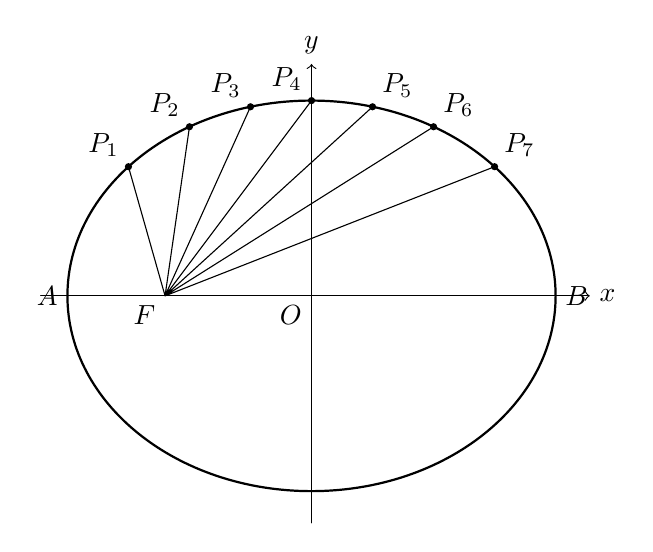
\begin{tikzpicture}[line cap=round,line join=round,x=0.62cm,y=0.62cm]
  \coordinate (P1) at (-3.75,2.646);
  \coordinate (P2) at (-2.50,3.464);
  \coordinate (P3) at (-1.25,3.873);
  \coordinate (P4) at (0,4);
  \coordinate (P5) at (1.25,3.873);
  \coordinate (P6) at (2.50,3.464);
  \coordinate (P7) at (3.75,2.646);
  \coordinate (F) at (-3,0);
  \draw[->] (-5.55,0)--(5.7,0) node[right] {$x$};
  \draw[->] (0,-4.65)--(0,4.75) node[above] {$y$};
  \draw[thick] (0,0) ellipse (5 and 4);
  \draw[thin] (F)--(P1) (F)--(P2) (F)--(P3) (F)--(P4)
              (F)--(P5) (F)--(P6) (F)--(P7);
  \foreach \i in {1,...,7} \fill (P\i) circle (1.3pt);
  \node[left] at (-5,0) {$A$};
  \node[right] at (5,0) {$B$};
  \node[below left] at (F) {$F$};
  \node[below left] at (0,0) {$O$};
  \node[above left] at (P1) {$P_1$};
  \node[above left] at (P2) {$P_2$};
  \node[above left] at (P3) {$P_3$};
  \node[above left] at (P4) {$P_4$};
  \node[above right] at (P5) {$P_5$};
  \node[above right] at (P6) {$P_6$};
  \node[above right] at (P7) {$P_7$};
\end{tikzpicture}
\end{center}
\nopagebreak[4]
\Needspace{4\baselineskip}
\textbf{解析}

椭圆半长轴 $a=5$，焦距参数 $c=3$。设八等分点横坐标为 $x_i=-5+\frac{10i}{8}$，$i=1,\ldots,7$，则 $\sum x_i=0$。对右焦点，各点焦半径为 $5-\frac35x_i$；对左焦点为 $5+\frac35x_i$。无论 $F$ 取哪一个焦点，七个焦半径之和均为 $7\cdot5=35$。

\gkanswer{答案：$35$}

\end{answer}
\begin{answer}
\gksolhead{16}{}

\textbf{题目}：

非空集合 $G$ 关于运算 $\oplus$ 满足：(1) 对任意 $a\text{、}b\in G$，都有 $a\oplus b\in G$；(2) 存在 $e\in G$，使得对一切 $a\in G$，都有 $a\oplus e=e\oplus a=a$，则称 $G$ 关于运算 $\oplus$ 为“融洽集”。现给出下列集合和运算：

① $G=\{\text{\text{非负整数}}\}$，$\oplus$ 为整数的加法；

② $G=\{\text{\text{偶数}}\}$，$\oplus$ 为整数的乘法；

③ $G=\{\text{\text{平面向量}}\}$，$\oplus$ 为平面向量的加法；

④ $G=\{\text{\text{二次三项式}}\}$，$\oplus$ 为多项式的加法；

⑤ $G=\{\text{\text{虚数}}\}$，$\oplus$ 为复数的乘法。

其中 $G$ 关于运算 $\oplus$ 为“融洽集”的是\gkblank{}。（写出所有“融洽集”的序号）

\Needspace{4\baselineskip}
\textbf{解析}

①非负整数对加法封闭且有单位元 $0$；③平面向量对加法封闭且有零向量单位元。②虽对乘法封闭，但单位元 $1$ 不属于偶数集。④多项式和虽可加，但二次三项式集不含零多项式，且相加可能消去二次项而不再是二次三项式。⑤虚数对乘法不封闭，例如 $i\cdot i=-1$ 为实数。因此只有①③。

\gkanswer{答案：①③}

\end{answer}
\begin{answer}
\gksolhead{17}{}

\textbf{题目}：

已知 $A\text{、}B\text{、}C$ 是 $\triangle ABC$ 三内角，向量 $\mathbf m=(-1,\sqrt3)$、$\mathbf n=(\cos A,\sin A)$，且 $\mathbf m\cdot\mathbf n=1$。

(1) 求角 $A$；

(2) 若 $\dfrac{1+\sin2B}{\cos^2B-\sin^2B}=-3$，求 $\tan C$。

\Needspace{4\baselineskip}
\textbf{解析}

\textbf{(1) 解析}

\Needspace{5\baselineskip}
由 $\mathbf m=(-1,\sqrt3)$ 与 $\mathbf n=(\cos A,\sin A)$ 的点积条件，
\nopagebreak[4]
\[
-\cos A+\sqrt3\sin A=1
=2\sin\left(A-\frac\pi6\right)\mbox{。}
\]
因 $A\in(0,\pi)$，方程 $\sin(A-\frac\pi6)=\frac12$ 的三角形内角解为 $A=\frac\pi3$（$A=\pi$ 不满足三角形内角条件）。

\textbf{(2) 解析}

\Needspace{5\baselineskip}
利用 $1+\sin2B=(\sin B+\cos B)^2$ 与 $\cos2B=(\cos B+\sin B)(\cos B-\sin B)$，原式在其有定义的范围内化为：
\nopagebreak[4]
\[
\frac{1+\tan B}{1-\tan B}=-3
\]
\Needspace{5\baselineskip}
得 $\tan B=2$。又 $C=\frac{2\pi}3-B$，故
\nopagebreak[4]
\[
\tan C=\tan\left(\frac{2\pi}3-B\right)
=\frac{-\sqrt3-2}{1-2\sqrt3}
=\frac{8+5\sqrt3}{11}\mbox{。}
\]

\gkanswer{答案（1）：$A=\dfrac\pi3$}

\gkanswer{答案（2）：$\tan C=\dfrac{8+5\sqrt3}{11}$}

\end{answer}
\begin{answer}
\gksolhead{18}{}

\textbf{题目}：

某课程考核分理论和实验两部分进行，每部分考核成绩只记“合格”与“不合格”，两部分考核都“合格”则该课程考核“合格”。甲、乙、丙三人在理论考核中合格的概率分别为 $0.9\text{、}0.8\text{、}0.7$；在实验考核中合格的概率分别为 $0.8\text{、}0.7\text{、}0.9$。所有考核是否合格互相之间没有影响。

(1) 求甲、乙、丙三人在理论考核中至少有两人合格的概率；

(2) 求这三人该课程考核都合格的概率。（结果保留三位小数）

\Needspace{4\baselineskip}
\textbf{解析}

\textbf{(1) 解析}

\Needspace{5\baselineskip}
理论考核至少两人合格的概率为
\nopagebreak[4]
\[
0.9\cdot0.8\cdot0.7+0.1\cdot0.8\cdot0.7+0.9\cdot0.2\cdot0.7+0.9\cdot0.8\cdot0.3=0.902\mbox{。}
\]

\textbf{(2) 解析}

甲、乙、丙课程考核合格概率分别为 $0.9\cdot0.8=0.72\text{、}0.8\cdot0.7=0.56\text{、}0.7\cdot0.9=0.63$。所有考核互相独立，故三人都合格的概率为 $0.72\cdot0.56\cdot0.63=0.254016\approx0.254$。

\gkanswer{答案（1）：$0.902$}

\gkanswer{答案（2）：$0.254$}

\end{answer}
\begin{answer}
\gksolhead{19}{}

\textbf{题目}：

如图，在长方体 $ABCD-A_1B_1C_1D_1$ 中，$E\text{、}P$ 分别是 $BC\text{、}A_1D_1$ 的中点，$M\text{、}N$ 分别是 $AE\text{、}CD_1$ 的中点，$AD=AA_1=a$，$AB=2a$。

(1) 求证：$MN\parallel$ 面 $ADD_1A_1$；

(2) 求二面角 $P-AE-D$ 的大小；

(3) 求三棱锥 $P-DEN$ 的体积。
\nopagebreak[4]
\begin{center}% 2006 四川理科 19：长方体 ABCD-A_1B_1C_1D_1 及题设中点、构造线
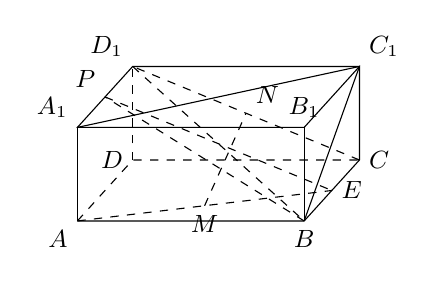
\begin{tikzpicture}[scale=0.9, font=\small]
  % 斜投影：AB=2a，AD=AA_1=a；比例仅用于示意。
  \coordinate (A)  at (0,0);
  \coordinate (B)  at (3.2,0);
  \coordinate (D)  at (0.78,0.86);
  \coordinate (C)  at (3.98,0.86);
  \coordinate (A1) at (0,1.32);
  \coordinate (B1) at (3.2,1.32);
  \coordinate (D1) at (0.78,2.18);
  \coordinate (C1) at (3.98,2.18);
  \coordinate (E)  at (3.59,0.43);
  \coordinate (P)  at (0.39,1.75);
  \coordinate (M)  at (1.795,0.215);
  \coordinate (N)  at (2.38,1.52);

  % 实线棱：前面、右侧及上部可见轮廓。
  \draw (A)--(B)--(C)--(C1)--(B1)--(A1)--(D1)--(C1);
  \draw (A)--(A1);
  \draw (B)--(B1);
  % 题图中的辅助线。
  \draw (A1)--(C1);
  \draw (B)--(C1);

  % 被遮挡的棱与位于后方/底面的构造线。
  \draw[dashed] (A)--(D)--(C);
  \draw[dashed] (D)--(D1);
  \draw[dashed] (A)--(E);
  \draw[dashed] (M)--(N);
  \draw[dashed] (P)--(E);
  \draw[dashed] (B)--(P);
  \draw[dashed] (D1)--(B);
  \draw[dashed] (C)--(D1);

  \node[below left] at (A) {$A$};
  \node[below] at (B) {$B$};
  \node[right] at (C) {$C$};
  \node[left] at (D) {$D$};
  \node[above left] at (A1) {$A_1$};
  \node[above] at (B1) {$B_1$};
  \node[above right] at (C1) {$C_1$};
  \node[above left] at (D1) {$D_1$};
  \node[above left] at (P) {$P$};
  \node[above right] at (N) {$N$};
  \node[below] at (M) {$M$};
  \node[right] at (E) {$E$};
\end{tikzpicture}
\end{center}
\nopagebreak[4]
\Needspace{4\baselineskip}
\textbf{解析}

\textbf{(1) 证明}

取坐标 $A=(0,0,0)\text{、}B=(2a,0,0)\text{、}D=(0,a,0)\text{、}A_1=(0,0,a)$。则 $C=(2a,a,0)\text{、}D_1=(0,a,a)$，$E=(2a,\frac a2,0)$，$M=(a,\frac a4,0)$，$N=(a,a,\frac a2)$。因此 $\overrightarrow{MN}=(0,\frac{3a}4,\frac a2)$，其方向向量的 $x$ 分量为 $0$，平行于平面 $ADD_1A_1$，故 $MN\parallel$ 平面 $ADD_1A_1$。

\textbf{(2) 解析}

取 $a=1$。平面 $DAE$ 为底面，其法向量为 $(0,0,1)$。平面 $PAE$ 的法向量可取 $\overrightarrow{AE}\times\overrightarrow{AP}=(\frac12,-2,1)$，模为 $\frac{\sqrt{21}}2$。两法向量夹角的余弦为 $\frac2{\sqrt{21}}$，即所求二面角大小为 $\arccos\frac2{\sqrt{21}}$。

\textbf{(3) 解析}

\Needspace{5\baselineskip}
仍取 $a=1$，用点 $D$ 为原点。则 $E-D=(2,-\frac12,0)$、$N-D=(1,0,\frac12)$、$P-D=(0,-\frac12,1)$。三棱锥体积为混合积绝对值的六分之一：
\nopagebreak[4]
\[
V_{P-DEN}=\frac16\left|\det\begin{pmatrix}2&-\frac12&0\\1&0&\frac12\\0&-\frac12&1\end{pmatrix}\right|=\frac16\mbox{。}
\]
恢复长度尺度 $a$ 后，体积为 $\frac{a^3}{6}$。

\gkanswer{答案（1）：$MN\parallel$ 平面 $ADD_1A_1$}

\gkanswer{答案（2）：$\arccos\dfrac2{\sqrt{21}}$}

\gkanswer{答案（3）：$\dfrac{a^3}{6}$}

\end{answer}
\begin{answer}
\gksolhead{20}{}

\textbf{题目}：

已知数列 $\{a_n\}$，其中 $a_1=1$，$a_2=3$，$2a_n=a_{n+1}+a_{n-1}\ (n\geqslant2)$。记数列 $\{a_n\}$ 的前 $n$ 项和为 $S_n$，数列 $\{\ln S_n\}$ 的前 $n$ 项和为 $U_n$。

(1) 求 $U_n$；

\Needspace{5\baselineskip}
(2) 设
\nopagebreak[4]
\[
F_n(x)=\frac{e^{U_n}}{2n(n!)^2}x^{2n}\quad(x>0),\qquad
T_n(x)=\sum_{k=1}^{n}F'_k(x)
\]
\Needspace{5\baselineskip}
（其中 $F'_k(x)$ 为 $F_k(x)$ 的导函数），计算
\nopagebreak[4]
\[
\lim_{n\to\infty}\frac{T_n(x)}{T_{n+1}(x)}\mbox{。}
\]

\Needspace{4\baselineskip}
\textbf{解析}

\textbf{(1) 解析}

\Needspace{5\baselineskip}
递推式等价于 $a_{n+1}-a_n=a_n-a_{n-1}$，故数列为等差数列。由 $a_1=1\text{、}a_2=3$ 得 $a_n=2n-1$，从而 $S_n=n^2$。于是
\nopagebreak[4]
\[
U_n=\sum_{j=1}^n\ln S_j=\sum_{j=1}^n\ln(j^2)=2\ln(n!)\mbox{。}
\]

\textbf{(2) 解析}

由 $e^{U_k}=(k!)^2$，得 $F_k(x)=\frac{x^{2k}}{2k}$，故 $F'_k(x)=x^{2k-1}$，且 $T_n(x)=\sum_{k=1}^n x^{2k-1}$。$0<x<1$ 时该和收敛到非零有限值，$x=1$ 时 $T_n=n$，两种情形比值极限均为 $1$。当 $x>1$ 时，$T_n/T_{n+1}\to x^{-2}$。

\gkanswer{答案（1）：$U_n=2\ln(n!)$}

\gkanswer{答案（2）：当 $0<x\leqslant1$ 时为 $1$；当 $x>1$ 时为 $\dfrac1{x^2}$}

\end{answer}
\begin{answer}
\gksolhead{21}{}

\textbf{题目}：

已知两定点 $F_1(-\sqrt2,0)\text{、}F_2(\sqrt2,0)$，满足条件 $|\overrightarrow{PF_2}|-|\overrightarrow{PF_1}|=2$ 的点 $P$ 的轨迹是曲线 $E$，直线 $y=kx-1$ 与曲线 $E$ 交于 $A\text{、}B$ 两点。如果 $|\overrightarrow{AB}|=6\sqrt3$，且曲线 $E$ 上存在点 $C$，使 $\overrightarrow{OA}+\overrightarrow{OB}=m\overrightarrow{OC}$，求 $m$ 的值和 $\triangle ABC$ 的面积 $S$。

\Needspace{4\baselineskip}
\textbf{解析}

\Needspace{5\baselineskip}
由 $|PF_2|-|PF_1|=2$ 知轨迹是双曲线 $x^2-y^2=1$ 的左支 $x\leqslant-1$。代入直线 $y=kx-1$，交点横坐标满足
\nopagebreak[4]
\[
(1-k^2)x^2+2kx-2=0\mbox{。}
\]
\Needspace{5\baselineskip}
要有两个不同的交点都在左支，需 $-\sqrt2<k<-1$。令 $u=k^2\in(1,2)$，弦长为
\nopagebreak[4]
\[
|AB|=\frac{2\sqrt{(2-u)(1+u)}}{u-1}\mbox{。}
\]
由 $|AB|=6\sqrt3$ 得 $28u^2-55u+25=0$，根为 $u=\frac54\text{、}\frac57$；只有 $u=\frac54$ 满足上述区间，故 $k=-\frac{\sqrt5}2$。

韦达定理给出 $x_A+x_B=-4\sqrt5$、$y_A+y_B=8$，所以 $\overrightarrow{OA}+\overrightarrow{OB}=(-4\sqrt5,8)$。由其等于 $m\overrightarrow{OC}$，可得 $C=(-\frac{4\sqrt5}{m},\frac8m)$。代入左支方程得 $m^2=16$，而 $x_C\leqslant-1$ 要求 $m>0$，故 $m=4$，$C=(-\sqrt5,2)$。

\Needspace{5\baselineskip}
点 $C$ 到直线 $y=-\frac{\sqrt5}{2}x-1$ 的距离为 $\frac13$，故
\nopagebreak[4]
\[
S_{\triangle ABC}=\frac12\cdot6\sqrt3\cdot\frac13=\sqrt3\mbox{。}
\]

\gkanswer{答案：$m=4$，$S=\sqrt3$}

\end{answer}
\begin{answer}
\gksolhead{22}{}

\textbf{题目}：

已知函数 $f(x)=x^2+\dfrac2x+a\ln x\ (x>0)$，$f(x)$ 的导函数是 $f'(x)$。对任意两个不相等的正数 $x_1\text{、}x_2$，证明：

\Needspace{5\baselineskip}
(1) 当 $a\leqslant0$ 时，
\nopagebreak[4]
\[
\frac{f(x_1)+f(x_2)}2>f\left(\frac{x_1+x_2}2\right);
\]

\Needspace{5\baselineskip}
(2) 当 $a\leqslant4$ 时，
\nopagebreak[4]
\[
|f'(x_1)-f'(x_2)|>|x_1-x_2|\mbox{。}
\]

\Needspace{4\baselineskip}
\textbf{解析}

\textbf{(1) 证明}

当 $a\leqslant0$ 时，$f''(x)=2+\frac4{x^3}-\frac a{x^2}>0$，所以 $f$ 在 $(0,\infty)$ 上严格凸。对不相等的 $x_1,x_2$，严格凸性给出两点函数值的平均严格大于中点处函数值。

\textbf{(2) 证明}

\Needspace{5\baselineskip}
当 $a\leqslant4$ 时，
\nopagebreak[4]
\[
f''(x)-1=\frac{x^3-ax+4}{x^3}\geqslant\frac{x^3-4x+4}{x^3}>0\mbox{。}
\]
\Needspace{5\baselineskip}
最后一个不等式成立，因为 $g(x)=x^3-4x+4$ 在 $x>0$ 的最小值取于 $x=2/\sqrt3$，且 $g(2/\sqrt3)=4-\frac{16}{3\sqrt3}>0$。由拉格朗日中值定理，存在介于 $x_1,x_2$ 的 $\xi$ 使
\nopagebreak[4]
\[
|f'(x_1)-f'(x_2)|=f''(\xi)|x_1-x_2|>|x_1-x_2|\mbox{。}
\]

\gkanswer{答案（1）：见解析版}

\gkanswer{答案（2）：见解析版}

\end{answer}